\documentclass[11pt]{beamer}
\usepackage[utf8]{inputenc}
\usepackage[T1]{fontenc}
\usepackage{lmodern}
\usetheme{Madrid}
\usepackage{tabularx}
\usepackage{booktabs}
\bibliographystyle{apalike}
%\usepackage[style=apa, backend=biber, natbib=true]{biblatex}
%\addbibresource{references.bib}
%\bibliography{document}
\begin{document}
	\author[Group Nine]{KALONG BONIFACE  - UEB3603118\\
		   FUGAH SELETEY MITCHELL  - UEB3602818\\
		  			  SUPERVISER: MR JUSTICE AMENYO KESSIE}  
\title[VARIABILITY CLIMATE CHANGE]{THE VARIABILITY CLIMATE CHANGE IS RESPONSIBLE FOR IN VEGETATION LOSS IN GHANA}
%	\subtitle{Quantifying The Status of Galamsey With Time Series Analysis}
	\logo{\includegraphics[scale=0.05]{images/logo2}}
	\institute[UENR]{Department of Mathematics and Statistics\\University Of Energy and Natural Resource,Sunyani}
	\date{\today}
	%\subject{Proposal}
	%\setbeamercovered{transparent}
	%\setbeamertemplate{navigation symbols}{}
	\begin{frame}
		\maketitle
	\end{frame}
	\begin{frame}
		\frametitle{Outline Of Presentation}
		\begin{itemize}
			\item Introduction
			\item Problem Statement
			\item Objective
			\item Methodology
			\item  Result  and Discussion
			\item Reference
		\end{itemize}
	\end{frame}

%	\begin{frame}
%		\frametitle{INTRODUCTION}
%		\begin{block}{}
%One would anticipate that the majority of emerging nations, which are still in the early stages of economic development and growth, would have a high forest cover and little deforestation. This, however, has not been the case. Ghana is a lower-middle-income nation that is still working toward middle-income classification. However, it has already begun to see a deforestation rate that is comparable to that of middle-income countries. The rapid population expansion, clearing of field for Galamsey operation,increased domestic need of wood for things like fuel, furniture, construction, and timber exports have all contributed to this trend, Bush fires in the 1980s, climate change, and lax law enforcement have all had an impact. \\
%       \end{block}
%	\end{frame}
%     \begin{frame}
%     	\frametitle{INTRODUCTION}
%     	\begin{block}{}
%     		The purpose of this paper is to establish an understanding in time series analysis on remotely sensed data. Which will introduced us to the fundamentals of time series modeling, including decomposition, autocorrelation and modeling historical changes in Galamsey Operation in Ghana, the Cause,Dangers and it's Environmental impact 
%     	\end{block}
%     
%     \end{frame}
 \begin{frame}
 	\frametitle{INTRODUCTION}
 	\begin{block}{}
 	One would anticipate that the majority of emerging nations, which are still in the early stages of economic development and growth, would have a high forest cover and little deforestation. This, however, has not been the case. Ghana is a lower-middle-income nation that is still working toward middle-income classification. However, it has already begun to see a deforestation rate that is comparable to that of middle-income countries. The rapid population expansion, clearing of field for Galamsey operation,increased domestic need of wood for things like fuel, furniture, construction, and timber exports have all contributed to this trend, Bush fires in the 1980s, climate change, and lax law enforcement have all had an impact.
 	
 	\end{block}
 	
 \end{frame}
%\begin{frame}
%	
%	\begin{block}{PROBLEM STATEMENT}
%		
%		The Footprint of Vegetation loss is Spreading at a very faster rate, causing vegetation loss.
%%		Other factors accounting to vegetation loss may largely include climate change,urban and exurban development, bush fires. But not much works or research has been done to tell the extent to which Galamsey causes vegetation loss. 
%		This research attempts to segregate the variability climate is responsible for in vegetation loss so as to attribute the residual variability to Galamsey and other related activities such as bush-fires etc.
%	
%	\end{block}
%\end{frame}
%\begin{frame}
%	\begin{block}{Research Questions}
%To address the challenge of the vegetation variability in this work, the following several statements were formed:
%
%\begin{itemize}
%	\item  Are there any changes in vegetation cause by Galamsey and Climate change in Ghana?
%	
%	\item Is there any relationship between vegetation and land surface temperature in Ghana?
%\end{itemize}
%	\end{block}
%\end{frame}
%\begin{frame}
%	\begin{block}{OBJECTIVE}
%	
%	The purpose is to establish an understanding in time series analysis on remotely sensed data. We will be introduced to the fundamentals of time series modeling, including decomposition, auto-correlation and modeling historical changes.
%	
%	\begin{itemize}
%		\item Perform time series analysis on satellite derived vegetation indices and Climatic Data
%		
%%		\item Estimate the extent to which Galamsey causes vegetation loss in Ghana.
%		
%		\item Dissociate or single out the variability climate is responsible for in vegetation loss
%	\end{itemize}
%	\end{block}
%\end{frame}
%\begin{frame}
%	\begin{block}{Significance Of The Study}
%		In this study, we want to examine the effects of climatic change on Ghana's vegetation during these thirty years.
%		
%		\begin{itemize}
%		\item 	This study allows us to explore climatic differences and climate-related drivers.
%		\item	It offers a chance to research how climatic variability affects the ecosystem and human health. 
%		\item	This study explores historical and projected vegetation and climate data, by sector, impacts, key vulnerabilities and what adaptation measures can be taken.
%		\item	It also explores the overview for a general context of how climate change is affecting Ghana.
%		\end{itemize}
%	\end{block}
%\end{frame}
\begin{frame}
		\begin{block}{PROBLEM STATEMENT}
			
			The Footprint of vegetation loss is spreading at a very faster rate, causing vegetation loss.
			%		Other factors accounting to vegetation loss may largely include climate change,urban and exurban development, bush fires. But not much works or research has been done to tell the extent to which Galamsey causes vegetation loss. 
			This research attempts to segregate the variability climate is responsible for in vegetation loss so as to attribute the residual variability to Galamsey and other related activities such as bush-fires etc.
			
		\end{block}
	\begin{block}{OBJECTIVE}
		
		%	The purpose is to establish an understanding in time series analysis on remotely sensed data. We will be introduced to the fundamentals of time series modeling, including decomposition, auto-correlation and modeling historical changes.
		
		\begin{itemize}
			\item Perform time series analysis on satellite derived vegetation indices and Climatic Data
			
			%		\item Estimate the extent to which Galamsey causes vegetation loss in Ghana.
			
			\item Dissociate or single out the variability climate is responsible for in vegetation loss
		\end{itemize}
	\end{block}
	\begin{block}{Limitation Of The Study}		
	
%The goal of time series modeling is to employ the simplest model feasible to account for as much data as possible while still developing an explanatory model of the data that does not over-fit the issue set.


\begin{itemize}
	\item Missing Data
%	\item It is almost certain that data from distant sensing will not provide the same level of precision.
	\item Atmospheric factors can distort the visual findings, causing the vegetation's color to shift dramatically from image to image as a result of atmospheric factors (fog, ground moisture, cloud cover)
\end{itemize}
	\end{block}
\end{frame}
\begin{frame}
	\frametitle{Data}
		
The Satellite (MOD13) provide consistent,and spatial time series comparisons of global vegetation conditions that can be used to monitor the Earth’s  photosynthetic vegetation activity in support of  \textbf{change detection}, and biophysical interpretations.For this analysis, we will be using the MOD13Q1 V6 product which contains the Enhanced Vegetation Index (EVI).
	% TODO: \usepackage{graphicx} required
	\begin{figure}
		\centering
		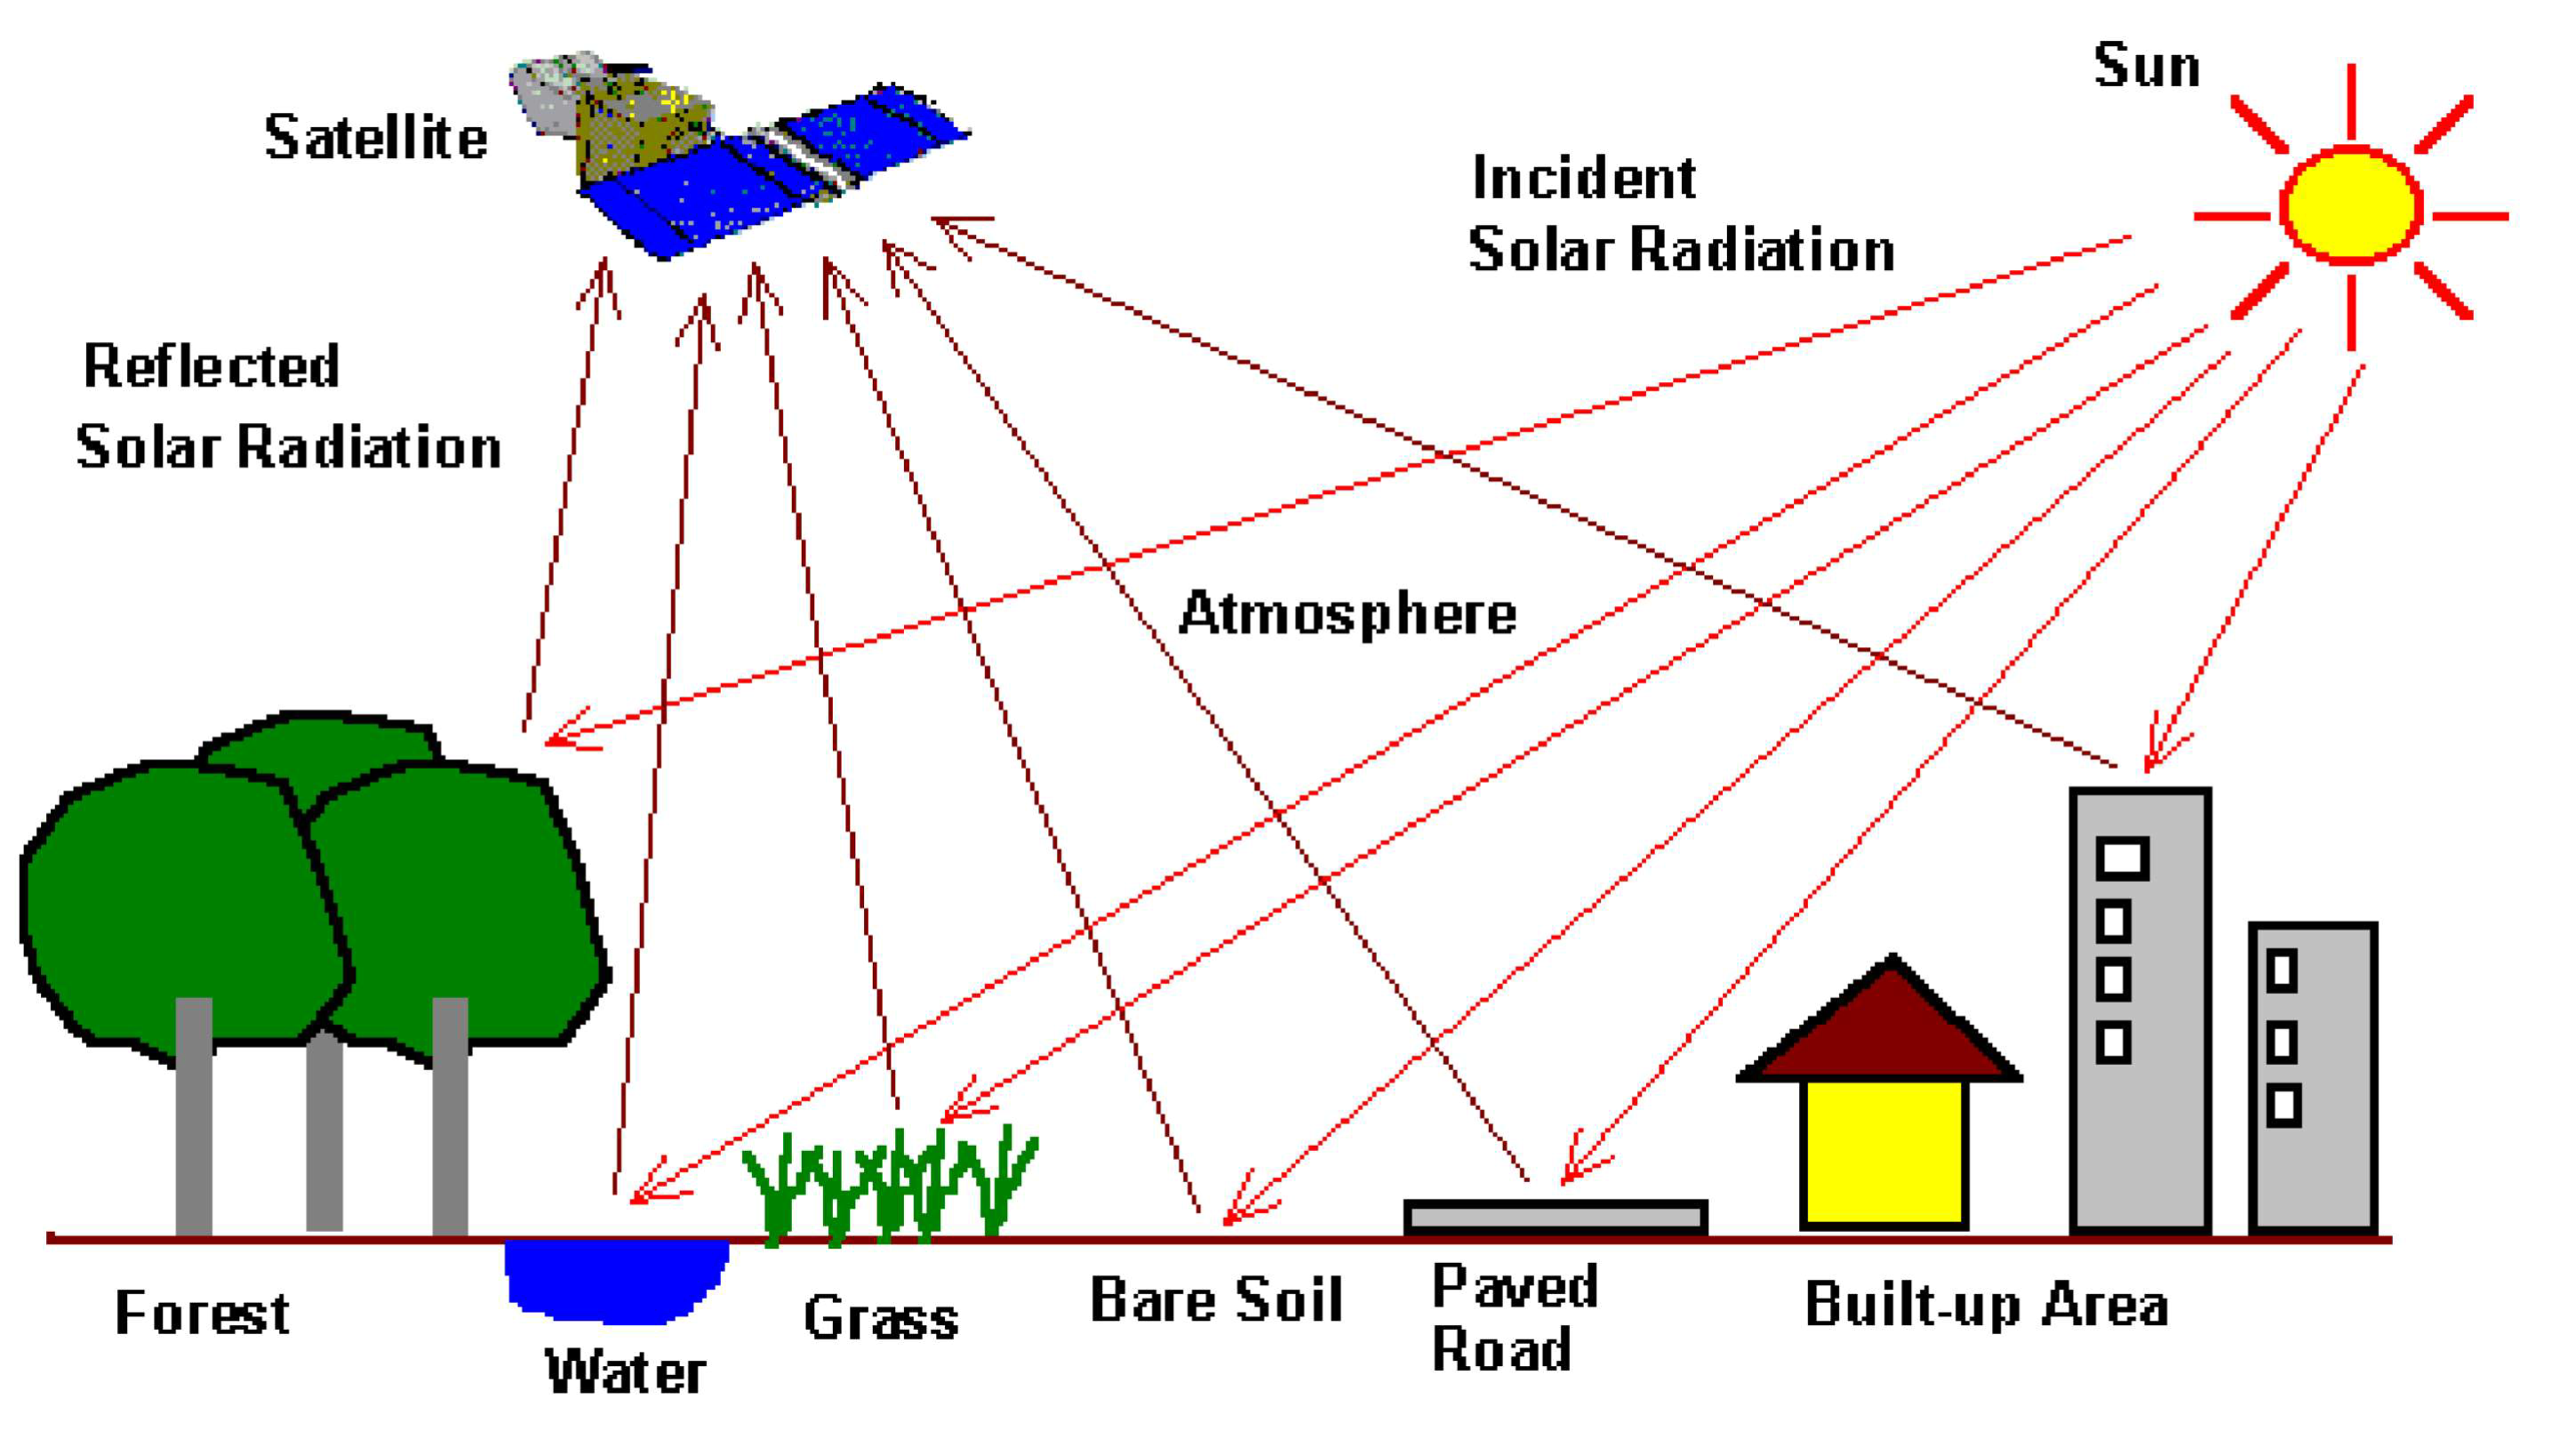
\includegraphics[width=0.7\linewidth]{images/classification}
		\caption{}
		\label{fig:classification}
	\end{figure}
	
\end{frame}

\begin{frame}
	\frametitle{Data}
% TODO: \usepackage{graphicx} required
\begin{equation}
	EVI = G\left[ \frac{NIR - Red}{NIR + C_{1}Red - C_{2}Blue + L}\right]
\end{equation}
	
\begin{itemize}
\item 	NIR, Red, and Blue are the surface reflectances that have been fully or partially adjusted
\item	C1 and C2 are the coefficients of the aerosol resistance term
\item	L is the canopy background adjustment for correcting the nonlinear, differential
\item   G is a gain or scaling factor. The MODIS EVI algorithm's chosen coefficients are
Where;  
		\begin{itemize}
			\item   L=1, C1=6, C2=7.5, and G=2.5.
		\end{itemize}
	
	\item  -1 $\leq$ EVI $\leq$1
\end{itemize}
	
\end{frame}
%\begin{frame}
%	\frametitle{Methodology-(Data Extraction)}
%	We will first collect data from Google Earth Engine in order to choose  EVI values and Climate Change data.
%	% TODO: \usepackage{graphicx} required
%	\begin{figure}
%		\centering
%		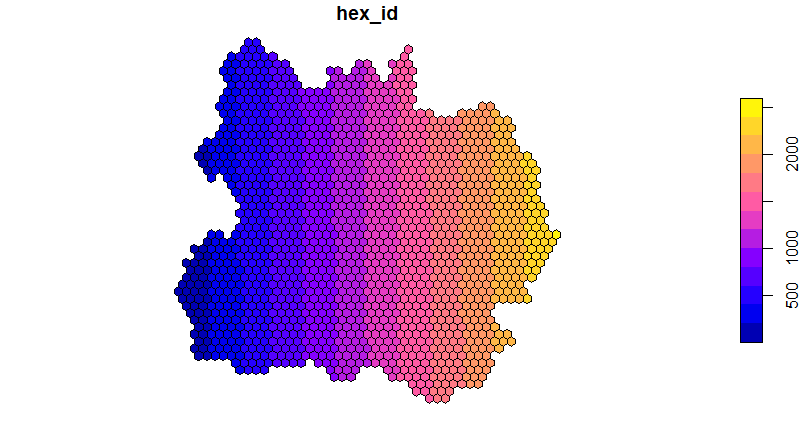
\includegraphics[width=0.7\linewidth]{images/Rplot}
%		\caption{Creating Hex cell(Polygons) on the Study Area}
%		\label{fig:rplot}
%	\end{figure}
%\end{frame}

\begin{frame}
	\frametitle{Data Extraction}
	% TODO: \usepackage{graphicx} required
	\begin{figure}
		\centering
		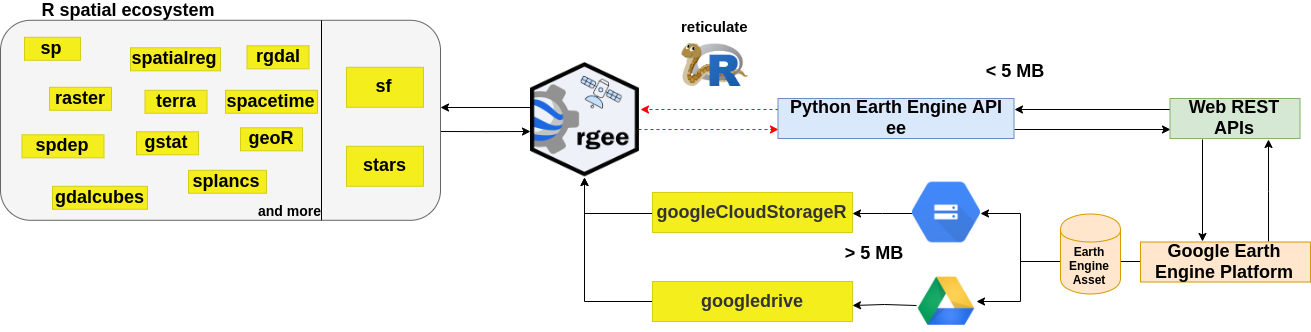
\includegraphics[width=0.7\linewidth]{images/DataExtraction}
		\caption{Data Extraction from Google Earth Engine}
		\label{fig:dataextraction}
	\end{figure}
	\begin{itemize}
			\item We will summarize the mean EVI values.
			\item We will apply a smoothing strategy using an ARIMA function to fix the situation where some cells may not have EVI for a particular month. 
			\item Eliminate seasonality before the normalized data is fitted using a linear model.
	\end{itemize}
\end{frame}

\begin{frame}{Data Visualization -(Univariate Analysis)}
	% TODO: \usepackage{graphicx} required
	\begin{figure}
		\centering
		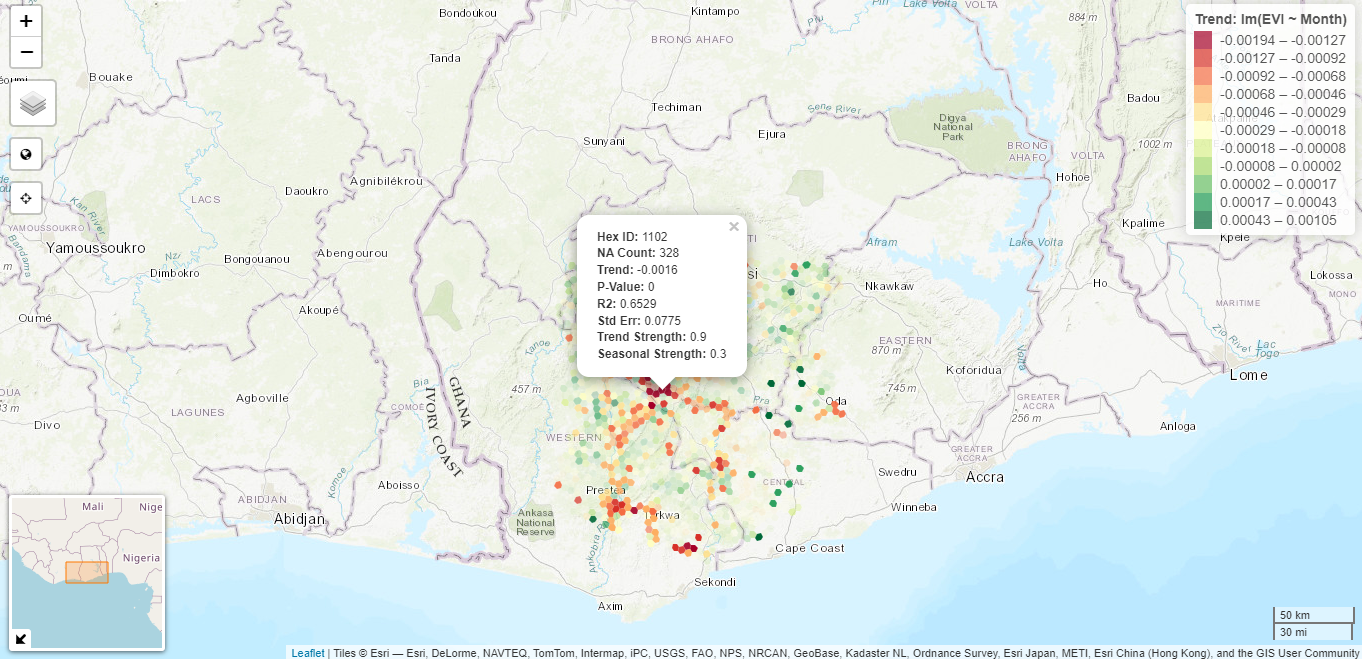
\includegraphics[width=1\textwidth,height=0.8\textheight]{images/Map}
		\caption{Vegetation Loss}
		\label{fig:map}
	\end{figure}
	
\end{frame}
\begin{frame}
	\begin{block}{Methodology -(Multivariate Analysis )}
		\begin{itemize}
		\item[*] To help machine learning classifiers works better with time series data .
		\item[*] Local features or patterns in time series can be found and combined to address challenges involving time-series categorization.
		\item[*] Then, a method to discover patterns that are helpful for classification is suggested.
		\item[*] Combine these patterns to create computable categorization rules. 
	\end{itemize}
\textbf{Vector Autoregression (VAR) }\\

It is of the form 
$y_{t} = A_{1}y_{t-1} + A_{2}y_{t-2} +\cdot+A_{p}y_{t-p}+ CD_{t} + \mu $\\
where;\\
\begin{itemize}
	\item  $ y_{t} = \left( y_{1t},y_{2t},...,y_{kt}\right)'$ is a vector of K observable endogenous variables \\
\item    For the purposes of this study, yt = $(EVI_{t}, Temperature_{t}, Rain_{}, Precipitation_{t},Drought_{t},Evaporation_{t})'$
\end{itemize}
 where EVI denotes the value of vegetation conditions  each month
	\end{block}
\end{frame}
\begin{frame}
	\frametitle{Structural Analysis (VAR)}
%	\begin{columns}
%		\begin{column}{0.5\textwidth}
			\begin{itemize}
				\item Augmented Dickey Fuller unit root test
				\item Lag Selection using information Criteria 
				   \begin{itemize}
				   \item	Akaike Information Criterion(AIC)
				   \item	Hannan-Quinn criterion(HQ)
				   \item Schwarz Criterion(SC)
				   \item Final Prediction Error criterion(FPE)
				   \end{itemize}
				\item Causality Test (Granger Causality)
				\item Impulse Response Analysis
				\item Forecast Error Variance Decomposition (FEVD)
			\end{itemize}
%		\end{column}
%		\begin{column}{0.5\textwidth}  %%<--- here
%					% TODO: \usepackage{graphicx} required
%					\begin{center}
%						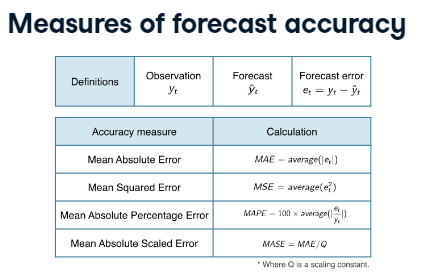
\includegraphics[width=0.7\linewidth]{images/Accuracy}
%					\end{center}
%		\end{column}
%	\end{columns}
\end{frame}
\begin{frame}{Result  (VAR TimeSeries Plot)}
% TODO: \usepackage{graphicx} required
\begin{figure}
	\centering
	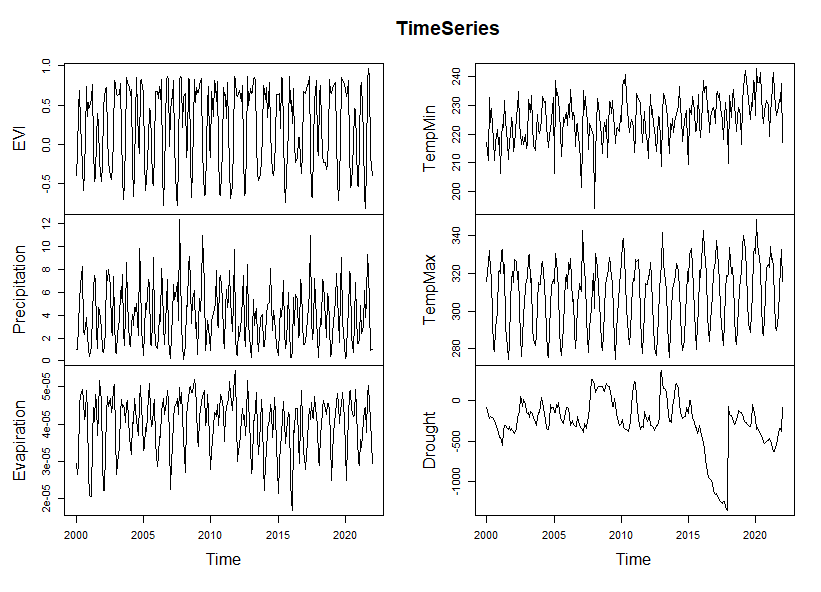
\includegraphics[width=0.7\linewidth]{images/TimeSeries}
	\caption{Time Series Plot}
	\label{fig:timeseries}
\end{figure}
\end{frame}
%\begin{frame}{Result }
%	\begin{itemize}
%		\item  $H_{0}$: "Process has unit root" vs. $H_{1}$: "Process has no unit root". 
%		\item Now we made comparison with the critical values under $H_{0}$
%	\end{itemize}
%	Since all the test statistic are much lower than all of the critical values we reject $H_{0}$ at a significance level   <1\%. So you can conclude with a very low probability of making an error that your time series has no unit root. So, We reject H0.
%\end{frame}
\begin{frame}{Result -(ADF) unit root test and(Granger Causality)}
	\begin{itemize}
		\item  $H_{0}$: "Process has unit root" vs. $H_{1}$: "Process has no unit root". 
		\item Now we made comparison with the critical values under $H_{0}$
	\end{itemize}
	Since all the test statistic are much lower than all of the critical values we reject $H_{0}$ at a significance level   <1\%. So you can conclude with a very low probability of making an error that your time series has no unit root. So, We reject $H_{0}$.
	\begin{table}[]
		\label{label:Optimal lag}
		\caption{Granger causality tests.}
		\centering
		\small
		\addtolength{\tabcolsep}{-4pt}
		\begin{tabularx}{\textwidth}{@{}lllll@{}}
			\hline
			Cause variable &Null hypothesis& F-value& p-value& Decision\\
			\hline\hline
			Precipitation	& does not Granger-cause EVI &2.1563  & 0.01464  & Reject the null hypothesis  \\
			\hline
			Evaporation	& does not Granger-cause EVI & 1.5398 & 0.1112 &Fail to Reject the null hypothesis  \\
			\hline
			TempMin	&  does not Granger-cause EVI&3.0049  & 0.0006276 &Reject the null hypothesis  \\
			\hline
			TempMax	& does not Granger-cause EVI&2.7462  & 0.001685 &Reject the null hypothesis  \\
			\hline
			Drought	& does not Granger-cause EVI & 0.9235 & 0.5241 &Fail to Reject the null hypothesis \\
			\hline
		\end{tabularx}
	\end{table}
\end{frame}
%\begin{frame}{Result}
%	% TODO: \usepackage{graphicx} required
%	\begin{figure}
%		\centering
%		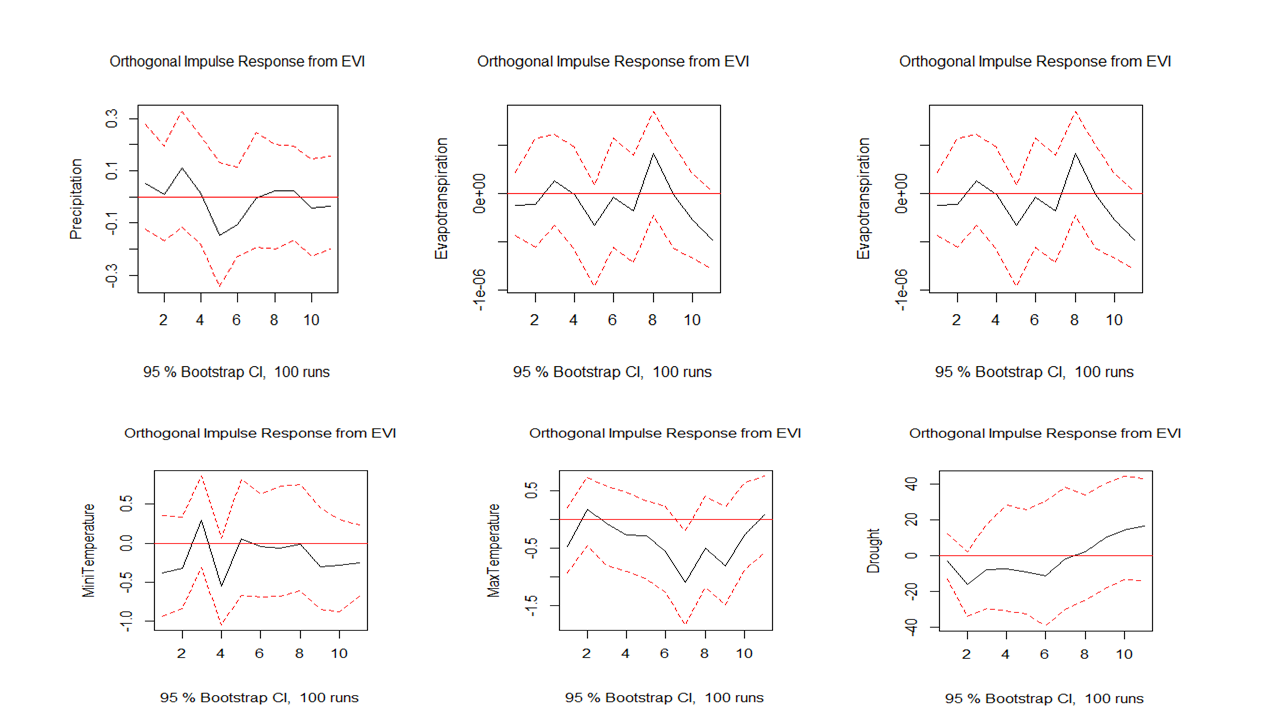
\includegraphics[width=0.7\linewidth]{images/impose}
%		\caption{}
%		\label{fig:impose}
%	\end{figure}
%	
%\end{frame}

%\begin{frame}{Result}
%	\begin{figure}
%		\centering
%		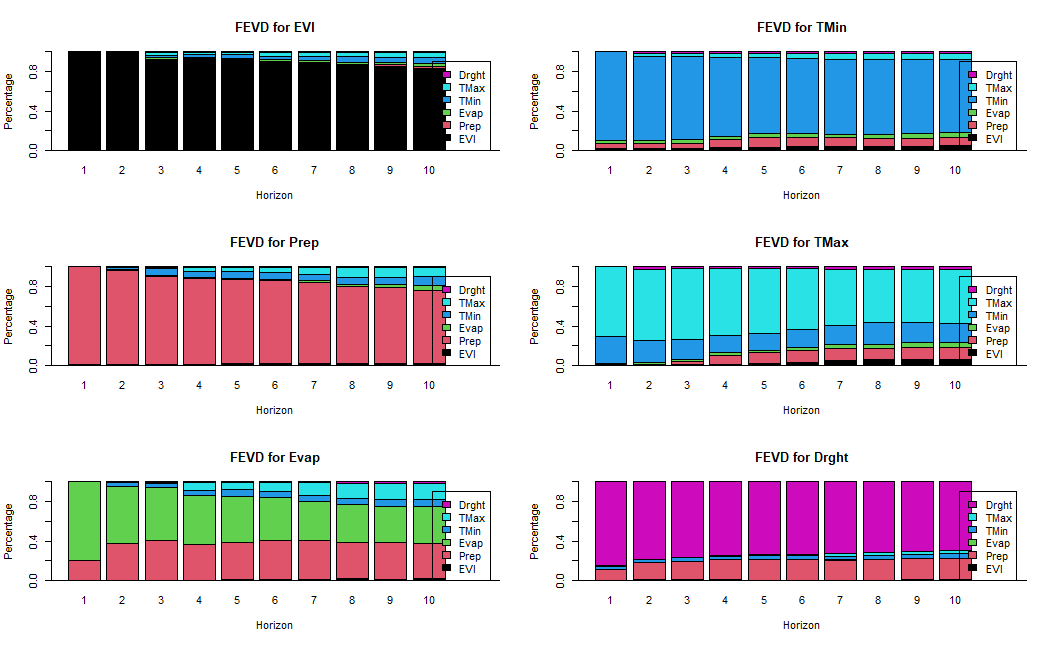
\includegraphics[width=0.7\linewidth]{images/fevd}
%		\caption{}
%		\label{fig:fevd}
%	\end{figure}
%\end{frame}
\begin{frame}{Result -(Forecast)}
% TODO: \usepackage{graphicx} required
\begin{figure}
	\centering
	\includegraphics[width=0.7\linewidth]{"images/FEVD and Forecast"}
	\caption{FEVD and Forecast}
	\label{fig:fevd-and-forecast}
\end{figure}

\end{frame}

\begin{frame}{}
        	\begin{table}[]
        			\label{table:Prediction}
        			\caption{EVI forecast for the next 12 month.}
        			\centering
        			\addtolength{\tabcolsep}{5pt}
        			\begin{tabularx}{\textwidth}{@{}lllll@{}}
        				\toprule
        				Month       & Forecast& Lower  &   Upper  &CI\\
        				\bottomrule
        		Feb 2022&-0.07548865& -0.65614302& 0.5051657& 0.5806544\\
        		Mar 2022& 0.14803164& -0.56646127& 0.8625245& 0.7144929\\
        		Apr 2022& 0.69105704& -0.04392727& 1.4260414& 0.7349843\\
        		May 2022& 0.72499702& -0.05679272& 1.5067868& 0.7817897\\
        		Jun 2022& 0.44066359& -0.41564183& 1.2969690& 0.8563054\\
        		Jul 2022&-0.11537243& -0.98453117& 0.7537863& 0.8691587\\
        		Aug 2022&-0.37165805& -1.24946226& 0.5061462& 0.8778042\\
        		Sep 2022&-0.16672258& -1.05855108& 0.7251059& 0.8918285\\
        		Oct 2022& 0.16015717& -0.73872579& 1.0590401& 0.8988830\\
        		Nov 2022&  0.37177202& -0.53806829& 1.2816123& 0.9098403\\
        				\bottomrule
        			\end{tabularx}
        	\end{table}   
\end{frame}
\begin{frame}{Accuracy and Discussion}
	\begin{table}
		\label{label: Accuracy}
		\caption{Forecast Accuracy on EVI Training set}
		\centering
		\small
		\addtolength{\tabcolsep}{-4pt}
		\begin{tabular}{llllllll}
			\hline\hline
		& ME	       & RMSE        &MAE          &MPE   &MAPE& MASE        &ACF1 \\
		              &-1.384005e-17& 2.665621e-01& 2.065071e-01&-Inf  &Inf & 0.00131& 0.0123\\
		\hline
\end{tabular}
\end{table}
	\begin{block}{}
		These findings are consistent with research by L.S Achille et al. They showed that maximum temperature and precipitation  particularly in the transition zone, was a better predictor of EVI trends than minimum Evaporation, although the findings of L.S Achille et al. show that Drought is not important.
	\end{block}
\end{frame}
\begin{frame}
	\frametitle{References}
	\begin{thebibliography}{9}
		\bibitem{Barenblitt, A. et al. (2021)} Science of the Total Environment 146644 (781).\\
		 \bibitem{H. L utkepohl,} Introduction to Multiple Time Series Analysis, Springer-Verlag, Berlin, Germany, 1993\\
%		\bibitem{H. Akaike,} “Canonical correlation analysis of time series anthe use of an information criterion,” in System Identification Advances and Case Studies, vol. 126 of Mathematics in Science and Engineering, pp. 27–96, Elsevier, 1976.\\
		\bibitem{D. A. Dickey and W. A. Fuller}, “Distribution of the estimators for autoregressive time series with a unit root,” Journal of the American Statistical Association, vol. 74, no. 366, pp. 427–431,1979.
	\end{thebibliography}
\end{frame}
\begin{frame}{}
	\begin{center}
		\Large\textbf{THANK YOU!}
	\end{center}
\end{frame}

\end{document}